\chapter{Modular and efficient Flock Pattern identification}
\label{chp:solution}
\section{Generic System Architecture}
\label{sec:architecture}
After the related work research that was performed, we noticed a lack of system architecture in order to solve data
spatio-temporal pattern detection problems. So far, no previous work has provide an architecture that could be easily
extensible and reusable for the myriad of the spatio-temporal pattern detection problems in the academy.

We first tried to approach this problem in a more generic fashion, since all moving pattern mining problem has the same
workflow:

\begin{enumerate}
    \item Connect to a spatio-temporal data source
    \item Retrieve and aggregate spatio-temporal data
    \item Process and mine that data in order to find the desired pattern or extract the desired information
\end{enumerate}

With that in mind, we designed a modular and easily extensible architecture that can fit for almost all spatio-temporal
data mining problem, which is depicted by \figref{fig:architecture}. One can notice that we focus on 4 key building
blocks, that can be easily registered/unregistered according to the targeting problem: (1) Data Source Connectors; (2)
Data Decoders; (3) Data Listeners (Data aggregators); (4) Data Processor.

In layer (1) we are concerned on how to retrieve the data, meaning how to communicate properly to the data source in
order to be able to extract each record of spatio-temporal data that the data source can provide. Thus, each "Data
Source Connector" (DSC) depicted in the \textit{Data Connectors' Module} in \figref{fig:architecture} represents a
logical piece that knows how to connect to and extract data from a specific data source. We can have a DSC that knows
how to connect to a MySQL database, or another one that can connect to a cloud based storage system like AWS DynamoDB,
or even a DSC that simply connects to an online data stream and listen for incoming data.

\begin{figure}[h!]
    \centering
    \caption{Generic System Architecture overview}
    \includegraphics[width=\linewidth]{images/architecture.png}
    \footnotesize{Source: Made by the author.}
    \label{fig:architecture}
\end{figure}

After connecting and retrieving data from a data source, we need to clean, decode and translate the incoming raw data to
a format that is simple and understandable to our system. To achieve that we will have a Data Decoder (DD) component,
which knows how to interpret the raw data format that comes from a DSC and translate it to a format that layer 3 can
understand. We can see in \figref{fig:architecture} that a DD can register itself to a DSC in order to receive each data
record that a DSC gathers from a data source. It is important to note that a DD can register to only one DSC, but a DSC
can have multiple DD registered to it.

In any problem of data mining, aggregation is one of the most important phases, since it is there that the data
gathering happens and necessary arrangements are made in order to get the data ready for processing. In our system that
is represented by layer (4), which we call the Data Listeners' Module. We can have multiple types of Data Listeners (DL)
in that module, and each of them can perform different types of aggregation and pre-processing depending on the final
goal.  For example, we could have an aggregator that bucketize the GPS points by their timestamp and filter out
outliers, before sending to processing, or another one that performs point interpolation in order to reduce trajectory
uncertainty. Similarly to the DD module, we can a DL can only register to one DD, but a DD can have multiple DL
registered to it. Later on we will see a DL proposed as one of the contributions by this dissertation, which will
perform a \textit{bufferized} aggregation of points.

The last, but not least, remaining piece is the Data Processors' Module, in layer (5). Is there that we will have the
intelligence to perform a data mining task that will generate insights for decision making, detect moving patterns and
the forth. We can have a Data Processor (DP) that detects flock patterns, other that detects convergence patterns and
other that provide traffic information in real time, to name a few. Following the pattern of the aforementioned modules,
each DP can only register to a single DL, but a DL can have multiple DPs registered to it. This dissertation will
present a novel DP for detecting flock patterns, based on the BFE algorithm proposed by Vieira et al. \citep{vieira}.

Researchers and data analysts can leverage from the proposed architecture in order to tackle multiple problems at once,
reusing components that can serve other spatio-temporal pattern mining problems.

\section{Aggregation and data processing efficiency}
\label{sec:bitdf}
By analyzing some of the algorithms proposed in \secref{sec:rel_flocks} and their respective running times, we noticed
that most of the CPU cycles were spent by analyzing disks that will not generate flock patterns, due to the points not
being present in $\delta$ consecutive time slots. In all algorithms, disks generated in time slot $t_{i+1}$ are compared
with those generated in $t_{i}$ in order to check if an extension to a potential flock pattern is found. This operation
has $O(nm)$ complexity, with $n$ being the number of disks and $m$ the number of potential flocks from previous time
slots.  Additionally, for each comparison between a disk and a potential flock, an intersection operation between them
needs to be made.

Things get even worse in algorithms like BFE, where a new created disk $D$ is checked if it is either subset or a
duplicate of a previously found disk (as already mentioned in \secref{subsec:disk_discovery}). The running time of this
step can result in a $O(n^2)$ time complexity in the worst case (with $n$ being the number of disks generated by that
time slot) requiring an intersection operation between each pair of disks that are being compared. We can reduce
significantly that number of disks by only creating disks with points that can potentially form a flock, i.e. with
points that appears in the dataset for $\delta$ consecutive time slots. We measured the time spent in those disk related
operations, using the datasets that we will use in our experiments, and showed the results in
\figref{fig:time_consumption}. There we can see that the disk and flock related operations can reach 99\% of the overall
processing time of the algorithm.

Consider the example depicted in Fig. \ref{fig:disks}, where we are looking for flocks with $\mu=4$ and $\delta=4$. As
we can see, in time slot $t_0$ our dataset reported points $p_1,p_2,p_3$ and $p_4$ and, due to the proximity between
them, disk $d_0$ was created enclosing all four points. In $t_1$ the same points were reported and again the regular
algorithm was able to create another disk $d_1$. However, in $t_2$, $p_3$ was not present and the disk $d_2$ only
contained three points, which is not enough to represent a flock pattern because the number of trajectories is less than
$\mu = 4$. Hence, we could avoid the creation of disks $d_0$ and $d_1$ if we would know in advance that $p_3$ was
missing in $t_2$, saving CPU cycles of disk comparisons in $t_0$ and $t_1$. We argue that when scaled to a dataset of
millions of records with real-time processing, that disk check for subsets and flock extension, in the regular
algorithms, will lead to severe degradation in performance. With that in mind, we can say with high confidence that
reducing the processing time spent with unnecessary disks that won't generate flock patterns, can dramatically reduce
the overall processing time of the algorithm.

\begin{figure}[h!]
    \centering
    \caption{Percentage of time spent between disk and flock processing tasks against other tasks in the algorithm}
    \centerline{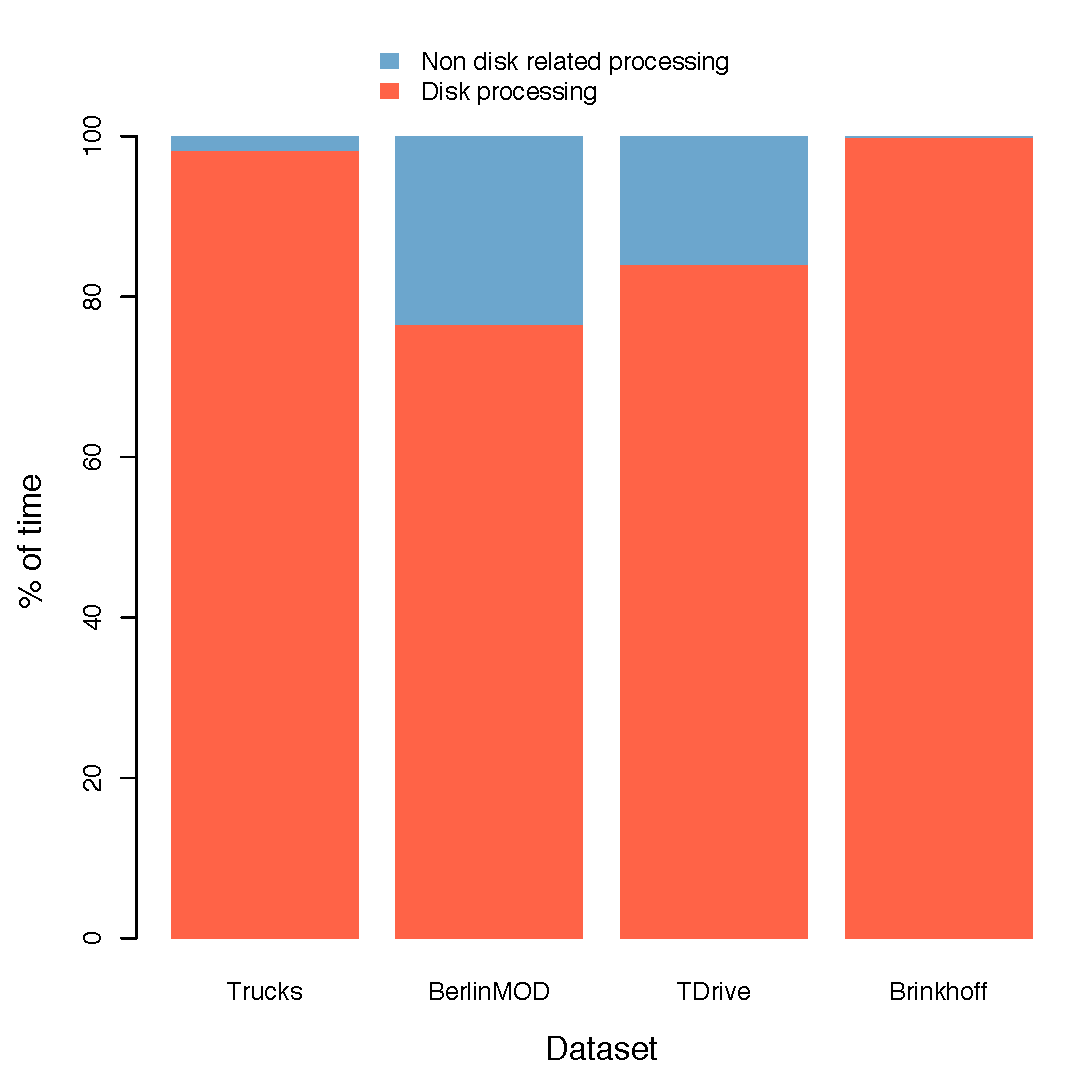
\includegraphics[width=0.7\linewidth]{images/timeConsumption.eps}}
    \footnotesize{Source: Made by the author.}
    \label{fig:time_consumption}
\end{figure}

\begin{figure}[h!]
    \centering
    \caption{Sequence of disks in 4 consecutive time slots and the points that were clustered to them}
    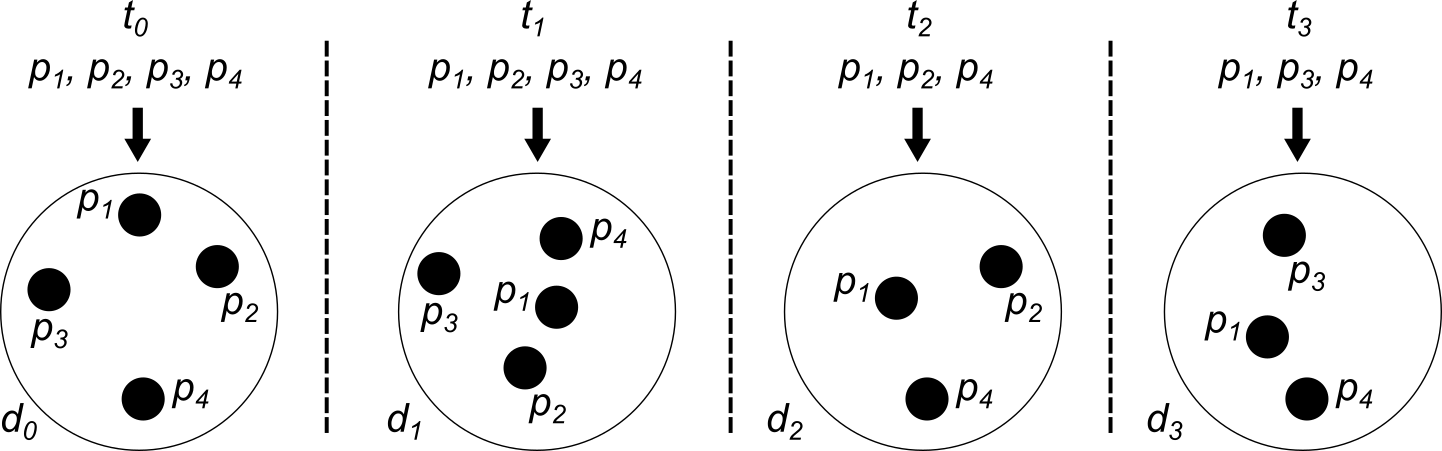
\includegraphics[width=\linewidth]{images/disks_2.png}
    \footnotesize{Source: Made by the author.}
    \label{fig:disks}
\end{figure}

\begin{algorithm}[h!]
\caption{GPS Stream Buffering}
\label{alg:gpsb}
\begin{algorithmic}[1]
    \State $pointBuffer \gets map\{index, \{id, point[...]\}\}$
    \State $presenceMap \gets map\{id, bitmap\}$
    \State $lastTimeslot \gets -1$
    \State
    \Procedure{AddPointPresence}{$id$}
        \State $mask \gets \Call{ShiftLeft}{1, pointBuffer.size - 1}$
        \State $presence \gets \Call{BitOr}{presenceMap[id], mask}$
        \State $presenceMap[id] \gets presence$
    \EndProcedure
    \State
    \Procedure{ShiftPresenceMaps}{}
        \ForAll {$id \in \Call{Keys}{presenceMap}$}
            \State $shifted \gets \Call{ShiftRight}{presenceMap[id], 1}$
            \State $presenceMap[id] \gets shifted$
        \EndFor
    \EndProcedure
    \State
    \Procedure{ReceivePoints}{}
        \Loop
            \State $point \gets gpsPointStream.dequeue$
            \State $timeSlot \gets point.timestamp / timeSlotSize$
            \If{$timeSlot > lastTimeslot$}
                \If{$pointBuffer.size \ge \delta$}
                    \State \Call{Fp.Process}{pointBuffer.first}
                    \State \textbf{delete} $pointBuffer.first$
                    \State \Call{ShiftPresenceMaps}{}
                \EndIf
                \State $lastTimeslot \gets timeSlot$
            \EndIf
            \State $pointBuffer[timeSlot][point.id].append(point)$
            \State \Call{AddPointPresence}{$point.id$}
        \EndLoop
    \EndProcedure
\end{algorithmic}
\end{algorithm}

Our solution consists on using \textbf{Bit}maps for \textbf{D}isk \textbf{F}iltering (BitDF), based on the BFE
algorithm. BitDF is basically a Data Listener and a Data Processor component, as those in the architecture presented in
\secref{sec:architecture}. We call them GPS Stream Buffering (GSB) and Flock Processor (FP) the DL and DP respectively,
and will have each of them keep track of the history of every $O_{id}$ in time.

Algorithm~\ref{alg:gpsb} shows a big picture of how GSB will work once it receives the point from a DD. It will listen
to the incoming GPS point stream in the procedure \textsc{ReceivePoints}, add each point to the \textit{pointBuffer}
structure (which is a hash map of points by time slot) and map each $O_{id}$ presence in time by calling
\textsc{AddPointPresence}. When GSB has buffered $\delta$ time slots (line 23) it will then send the points of $timeSlot
- \delta$ to FP. After FP is done with its processing, GSB will discard the first position of the presence maps (whic
corresponds to the points sent to FP), by calling \textsc{ShiftPresenceMaps}, and also discard the points collected in
$timeSlot - \delta$, which were already processed by FP. The flow continues indefinitely by buffering the points from
the next time slot $t_i$ and send the points from $t_{i - \delta}$ to FP for processing. It is worth noting
\textit{timeSlotSize} (line 21) refers to the time slot $\sigma$ introduced in \secref{sec:tech_data}.

Using Fig. \ref{fig:disks} as an example, we can see in \tabref{tab:bitmaps} the state of the GSB bitmaps for each
$O_{id}$ after receiving the points in $t_3$. With those bitmaps, we can easily look up for a specific point occurrence
in time and check if that point in that specific time slot can potentially form a flock pattern or not (if that $O_{id}$
appears for $\delta$ consecutive time slots in the dataset). The bitmaps in GSB will always refer to the "future" of a
specific $O_{id}$.

\begin{table}[h!]
    \renewcommand{\arraystretch}{1.3}
    \caption{Bitmaps in GSB after buffering four time slots}
    \label{tab:bitmaps}
    \centering
    \begin{tabular}{c|c}
        \hline
        $O_{id}$ &   Bitmap\\
        \hline
        \hline
        1        &   1111\\
        \hline
        2        &   0111\\
        \hline
        3        &   1011\\
        \hline
        4        &   1111\\
        \hline
    \end{tabular}
\end{table}

Our DP is explained in more detail by Algorithms~\ref{alg:fp_helpers} and~\ref{alg:fp} as follows. In
Algorithm~\ref{alg:fp_helpers} we start by first listing the procedures that will help the core procedure of FP (the
\textsc{Process} procedure, in Algorithm~\ref{alg:fp}). It is also in Algorithm~\ref{alg:fp_helpers} that we list the
most important piece of this DP that allows us to achieve such good optimizations, in both CPU cycles and number of
disks generated, which is the \textsc{IsPointEligible} procedure. Such procedure is responsible to put together what
happened in the \textit{past} and what is going to happen in the \textit{future} for a given point $p$, in order to
decide whether $p$ can be part of a potential flock pattern or not. It does that by concatenating, for a given $O_{id}$,
the bitmap from FP with the bitmap from GSB (line 5 of Algorithm~\ref{alg:fp_helpers}) and searching for a sequence of
$\delta$ bits set to 1 (lines 6 to 15 of Algorithm~\ref{alg:fp_helpers}). That search is performed by combining AND and
XOR bitwise operations against the presence bitmap assembled in line 5 of Algorithm~\ref{alg:fp_helpers}. If a sequence
of $\delta$ bits set to 1 is found, we can state with confidence that that point can potentially be part of a flock
pattern. Later on, if a potential flock is found in a time slot $t_i$ and $p$ is part of it, we need to update the FP's
bitmap of that point so when we process points of time slot $t_{i+1}$ we have the correct bitmap representation of $p$
and that is where \textsc{MapPointFlock} (line 20) comes to play. \textsc{MapPointFlock} does that by prepending 1 to
$p$'s bitmap in FP module by performing an OR bitwise operation.

\begin{algorithm}
\caption{Flock Processor Helper Procedures}
\label{alg:fp_helpers}
\begin{algorithmic}[1]
    \State $buffered \gets 0$ \Comment max time span of the current flocks, max value is $\delta$
    \State $flockMap \gets map\{id, bitmap\}$
    \State
    \Procedure{IsPointEligible}{$id$}
        \State $presence \gets \Call{Concat}{presenceMap[id], flockMap[id]}$
        \State $eligibleMask \gets \Call{ShiftLeft}{1, \delta} - 1$
        \State $range \gets pointBuffer.size + buffered$
        \State $checks \gets \Call{Max}{1, range - \delta + 1}$
        \While{$checks > 0$}
            \State $tmp \gets \Call{BitAnd}{presence, eligibleMask}$
            \If{\Call{BitXor}{$tmp, eligibleMask$}}
                \State \Return $\textbf{\textit{true}}$
            \EndIf
            \State $checks \gets checks - 1$
            \State $eligibleMask \gets \Call{ShiftLeft}{eligibleMask, 1}$
        \EndWhile
        \State \Return $\textbf{\textit{false}}$
    \EndProcedure
    \State
    \Procedure{MapPointFlock}{$id$}
        \State $mask \gets \Call{ShiftLeft}{1, buffered}$
        \State $flockMap[id] \gets \Call{BitOr}{flockMap[id, mask}$
    \EndProcedure
    \State
    \Procedure{ShiftFlockMaps}{}
        \ForAll {$id \in \Call{Keys}{flockMap}$}
            \State $flockMap[id] \gets \Call{ShiftRight}{flockMap[id], 1}$
        \EndFor
    \EndProcedure
    \State
    \Procedure{StoreDiskIfEligible}{$diskSet, d$}
        \If{$\Call{Count}{d} \ge \mu \enspace \textbf{and} \enspace \textbf{not} \enspace \Call{SubSet}{d}$}
            \State \Call{AddDisk}{$diskSet, d$}
        \Else
            \State \textbf{delete} $d$
        \EndIf
    \EndProcedure
\end{algorithmic}
\end{algorithm}

\begin{algorithm}
\caption{Flock Processor Process Procedure}
\label{alg:fp}
\begin{algorithmic}[1]
    \Procedure{Process}{$pointMap\{id, point[...]\}, timeslot$}
        \State $D \gets \emptyset$
        \State $cells \gets \Call{BuildGrid}{pointMap}$
        \If{$buffered \ge \delta$}
            \State \Call{ShiftFlockMaps}{}
            \State $buffered \gets buffered - 1$
        \EndIf
        \ForAll{$c_{x, y} \in cells$}
            \State $cellRange \gets [c_{x - 1, y - 1}...c_{x + 1, y+ 1}]$
            \ForAll{$p1 \in c_{x, y}$}
                \ForAll{$p2 \in cellRange$}
                    \If{$d(p1, p2) \le \epsilon$}
                        \State $d1, d2 \gets \Call{CreateDisks}{p1, p2}$
                        \ForAll{$p \in cellRange$}
                            \State $added \gets \textbf{false}$
                            \If{$\Call{InDisk}{d1, p} \enspace \textbf{and} \enspace \Call{IsPointEligible}{p}$}
                                \State $\Call{Add(d1, p)}$
                                \State $added \gets \textbf{true}$
                            \EndIf
                            \If{$\Call{InDisk}{d2, p} \enspace \textbf{and} \enspace \Call{IsPointEligible}{p}$}
                                \State $\Call{Add(d2, p)}$
                                \State $added \gets \textbf{true}$
                            \EndIf
                            \If{$added = \textbf{true}$}
                                \State $\Call{MapPointFlock}{p.id}$
                            \EndIf
                        \EndFor
                        \State \Call{StoreDiskIfEligible}{$D, d1$}
                        \State \Call{StoreDiskIfEligible}{$D, d2$}
                    \EndIf
                \EndFor
            \EndFor
        \EndFor
        \State $buffered \gets buffered + 1$
    \EndProcedure
\end{algorithmic}
\end{algorithm}

\figref{fig:gsb_fp_flow} shows how GSB (red) and FP (gray) will interact in a scenario where $\mu = 3$ and $\delta = 3$.
In the first line we can see GSB receiving points $p_1$, $p_2$, $p_3$, $p_4$ and $p_5$ at time slot $t_0$ and then
updating the bitmap for each of the points (red grid). Later on, at time slot $t_1$, GSB receives points $p_2$, $p_3$,
$p_4$, $p_5$ and $p_6$ and again updates the presence bitmaps for each point. After the bitmap updates, one can notice
that now $p_1$ has $01$ as its presence bitmap value, meaning that it was present at time slot $t_0$ but not at $t_1$,
and GSB now has a buffer of points for time slot $t_0$ (red dashed box). When the points from time slot $t_2$ are
received, and the presence bitmaps are updated, GSB send the points buffered from time slot $t_0$ to FP for processing.
At this time, FP hasn't received any set of points for processing, so its bitmaps are clean (rightmost gray grid) and
the concatenation of the bitmaps from GSB and FP will have the same value as in GSB. Ater processing the buffered points
from time slot $t_0$, FP will generate a disk $d_1$ with points $p_2$, $p_4$ and $p_5$, leaving $p_1$ and $p_6$ out
because their bitmaps say that they will not appear in the next 2 consecutive time slots.

\begin{figure}[h!]
    \centering
    \caption{Interaction between GSB (red) and FP (gray) in 5 consecutive time slots, showing how the presence bitmaps
        are constructed. In the example we have $\mu = 3$ and $\delta = 3$}
    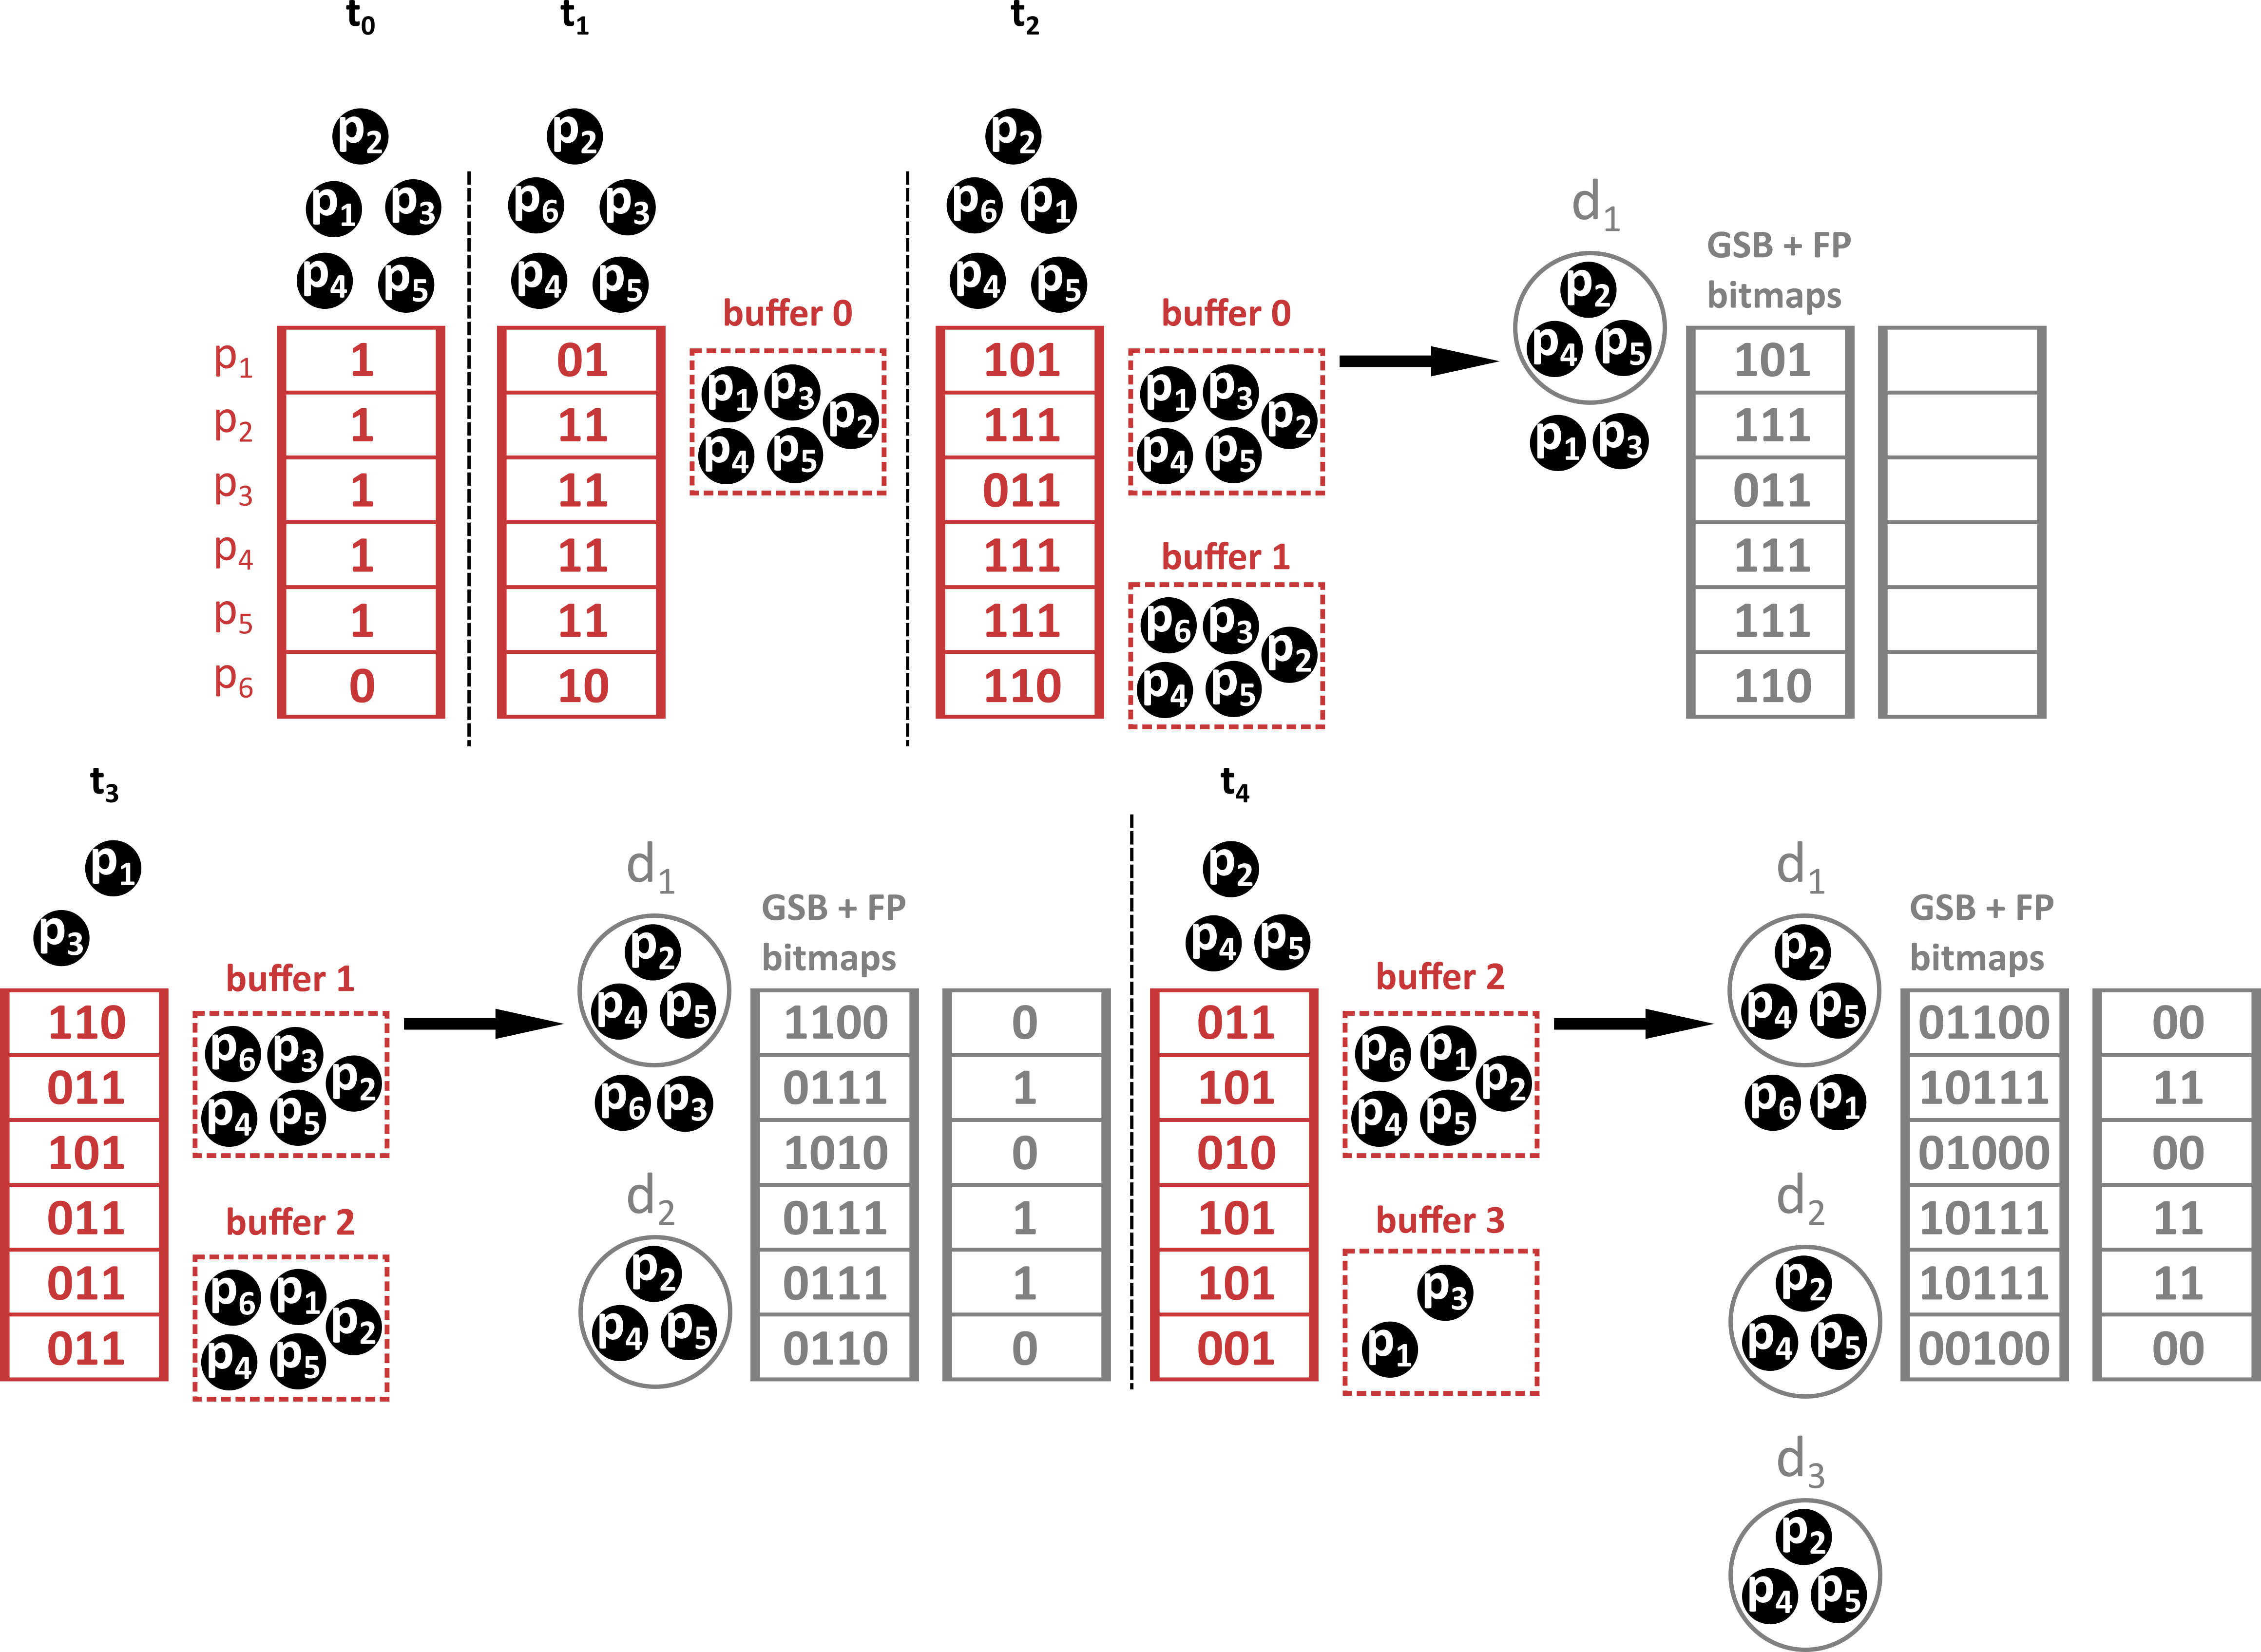
\includegraphics[width=\linewidth]{images/gsb_fp_flow.png}
    \footnotesize{Source: Made by the author.}
    \label{fig:gsb_fp_flow}
\end{figure}

The same flow continues for time slot $t_3$, with GSB sending the buffered points from time slot $t_1$ to FP for
processing. We can now notice that the points that formed disk $d_1$ in the time slot $t_0$ now have a bit set to 1 in
their presence bitmaps in FP. It is worth noting how we perform the bitmap concatenation in FP (when it receives points
from $t_1$), in which the past time (FP bitmaps) goes at the right and the future (GSB bitmaps) goes at the left side of
the concatenated bitmap. We then perform a search for $\mu = 3$ bits set to 1 in that concatenated bitmaps to figure out
which points can potentially form a flock and can be places in a disk.

In time slot $t_4$, when FP receives the points from time slot $t_2$, a flock pattern will be found, since we could find
3 disks containing the same set of $O_{id}$ and containing at least $\mu = 3$ unique $O_{id}$.

\section{Taking advantage of Multi-core Architectures}
\label{sec:multithread}
Is well known that multi-core architectures are the current trend in technology. There is a myriad of multi-core
processors in the market and many chipset companies taking advantages of those processor architectures too (even small
devices, like smartphones, are being shipped with multi-core processors). Given that current scenario, there is no
excuse in not taking advantage of those mult-core processors and still executing our solution in a single process
fashion. Thus, we will remodel our propoesed architecture and in a multi-threaded structure and parallelize the tasks
that our algorithm is doing, in order to make it more responsive and fast so it can empower decision makers to act in
realtime.

One can see that the FP component, that we described in the previous section, is doing a lot of work in order to
discover the flock patterns, whenever it receives the set of points from the listener it perform the following actions:

\begin{enumerate}
    \item Build the whole point grid
    \item For each grid cell:
    \begin{enumerate}
        \item Get the Extended Grid Cell (EGC) (e.g. for cell $c_{x,y}$ it will get cells
            $c_{x - 1, y - 1}...c_{x + 1, y+ 1}$)
        \item Process the EGC, trying to cluster the points in disks
    \end{enumerate}
    \item Get the resulting disks and assure that there are no duplicates nor subsets of other disks
    \item Try to merge the disks with potential flocks from previous time slots
    \item Report new found flocks
\end{enumerate}

It can be easily perceived that the EGC processing (steps (a) and (b)) can be done in parallel for the multiple cells
that will be processed, since there is no dependency concurrent writing operations between cells. Another step that is
very CPU heavy is the one described in step 3, but that one is very difficult to parallelize, as we could see in
Algorithm~\ref{alg:fp}. In that algorithm we showed that we start with an empty set of disks in the beginning of the
\textsc{Process} procedure and add disks to that set as we go finding them. However, before adding a disk $d$ we check,
amongst the other disks that were previously there, if $d$ is neither a subset nor a superset of an existing disk. If
$d$ is a subset, than it is not added, but if $d$ is superset of an existing disk $d_2$, that disk $d_2$ is then removed
from the set and $d$ is added instead (the superset check is done inside the procedure \textsc{AddDisk}). Thus, if we
try to parallelize that disk check procedure we would need to have synchronizing primitives to protect the concurrent
writing operations to the shared disk set, which could end up being more slow than executing it sequentially. Even
without being able to fully parallelize the disk check steps we can still take advantage of other techniques to gain
some speed in processing, like using the divide and conquer approach. The idea would be to have multiple disks sets (one
per independent worker thread processing EGCs) and have each independent thread add disks (and thus check for
subsets/supersets) to its own set. When each worker thread has finished its processing we would have each thread's set
being merged with the global disk set in FP. leaving less checks to be performed by the global disk set.

\subsection{Multi-threaded Design}
\label{subsec:multithread}
The multi-threaded idea described in \secref{sec:multithread} can be modeled as a Producer-Multiple Consumers problem,
where we would have a single producer assembling the EGCs and multiple consumers taking a EGC from a shared queue and
clustering the points in the disks that it might find in that specific EGC. On a step further, each consumer thread
$c_t$ will also spawn another thread $d_t$ that will process disks that $c_t$ has found and will check for subsets and
supersets in its own private disk set.

\begin{figure}[h!]
    \centering
    \caption{Modeling the FP in a Producer-Multiple Consumers architecture}
    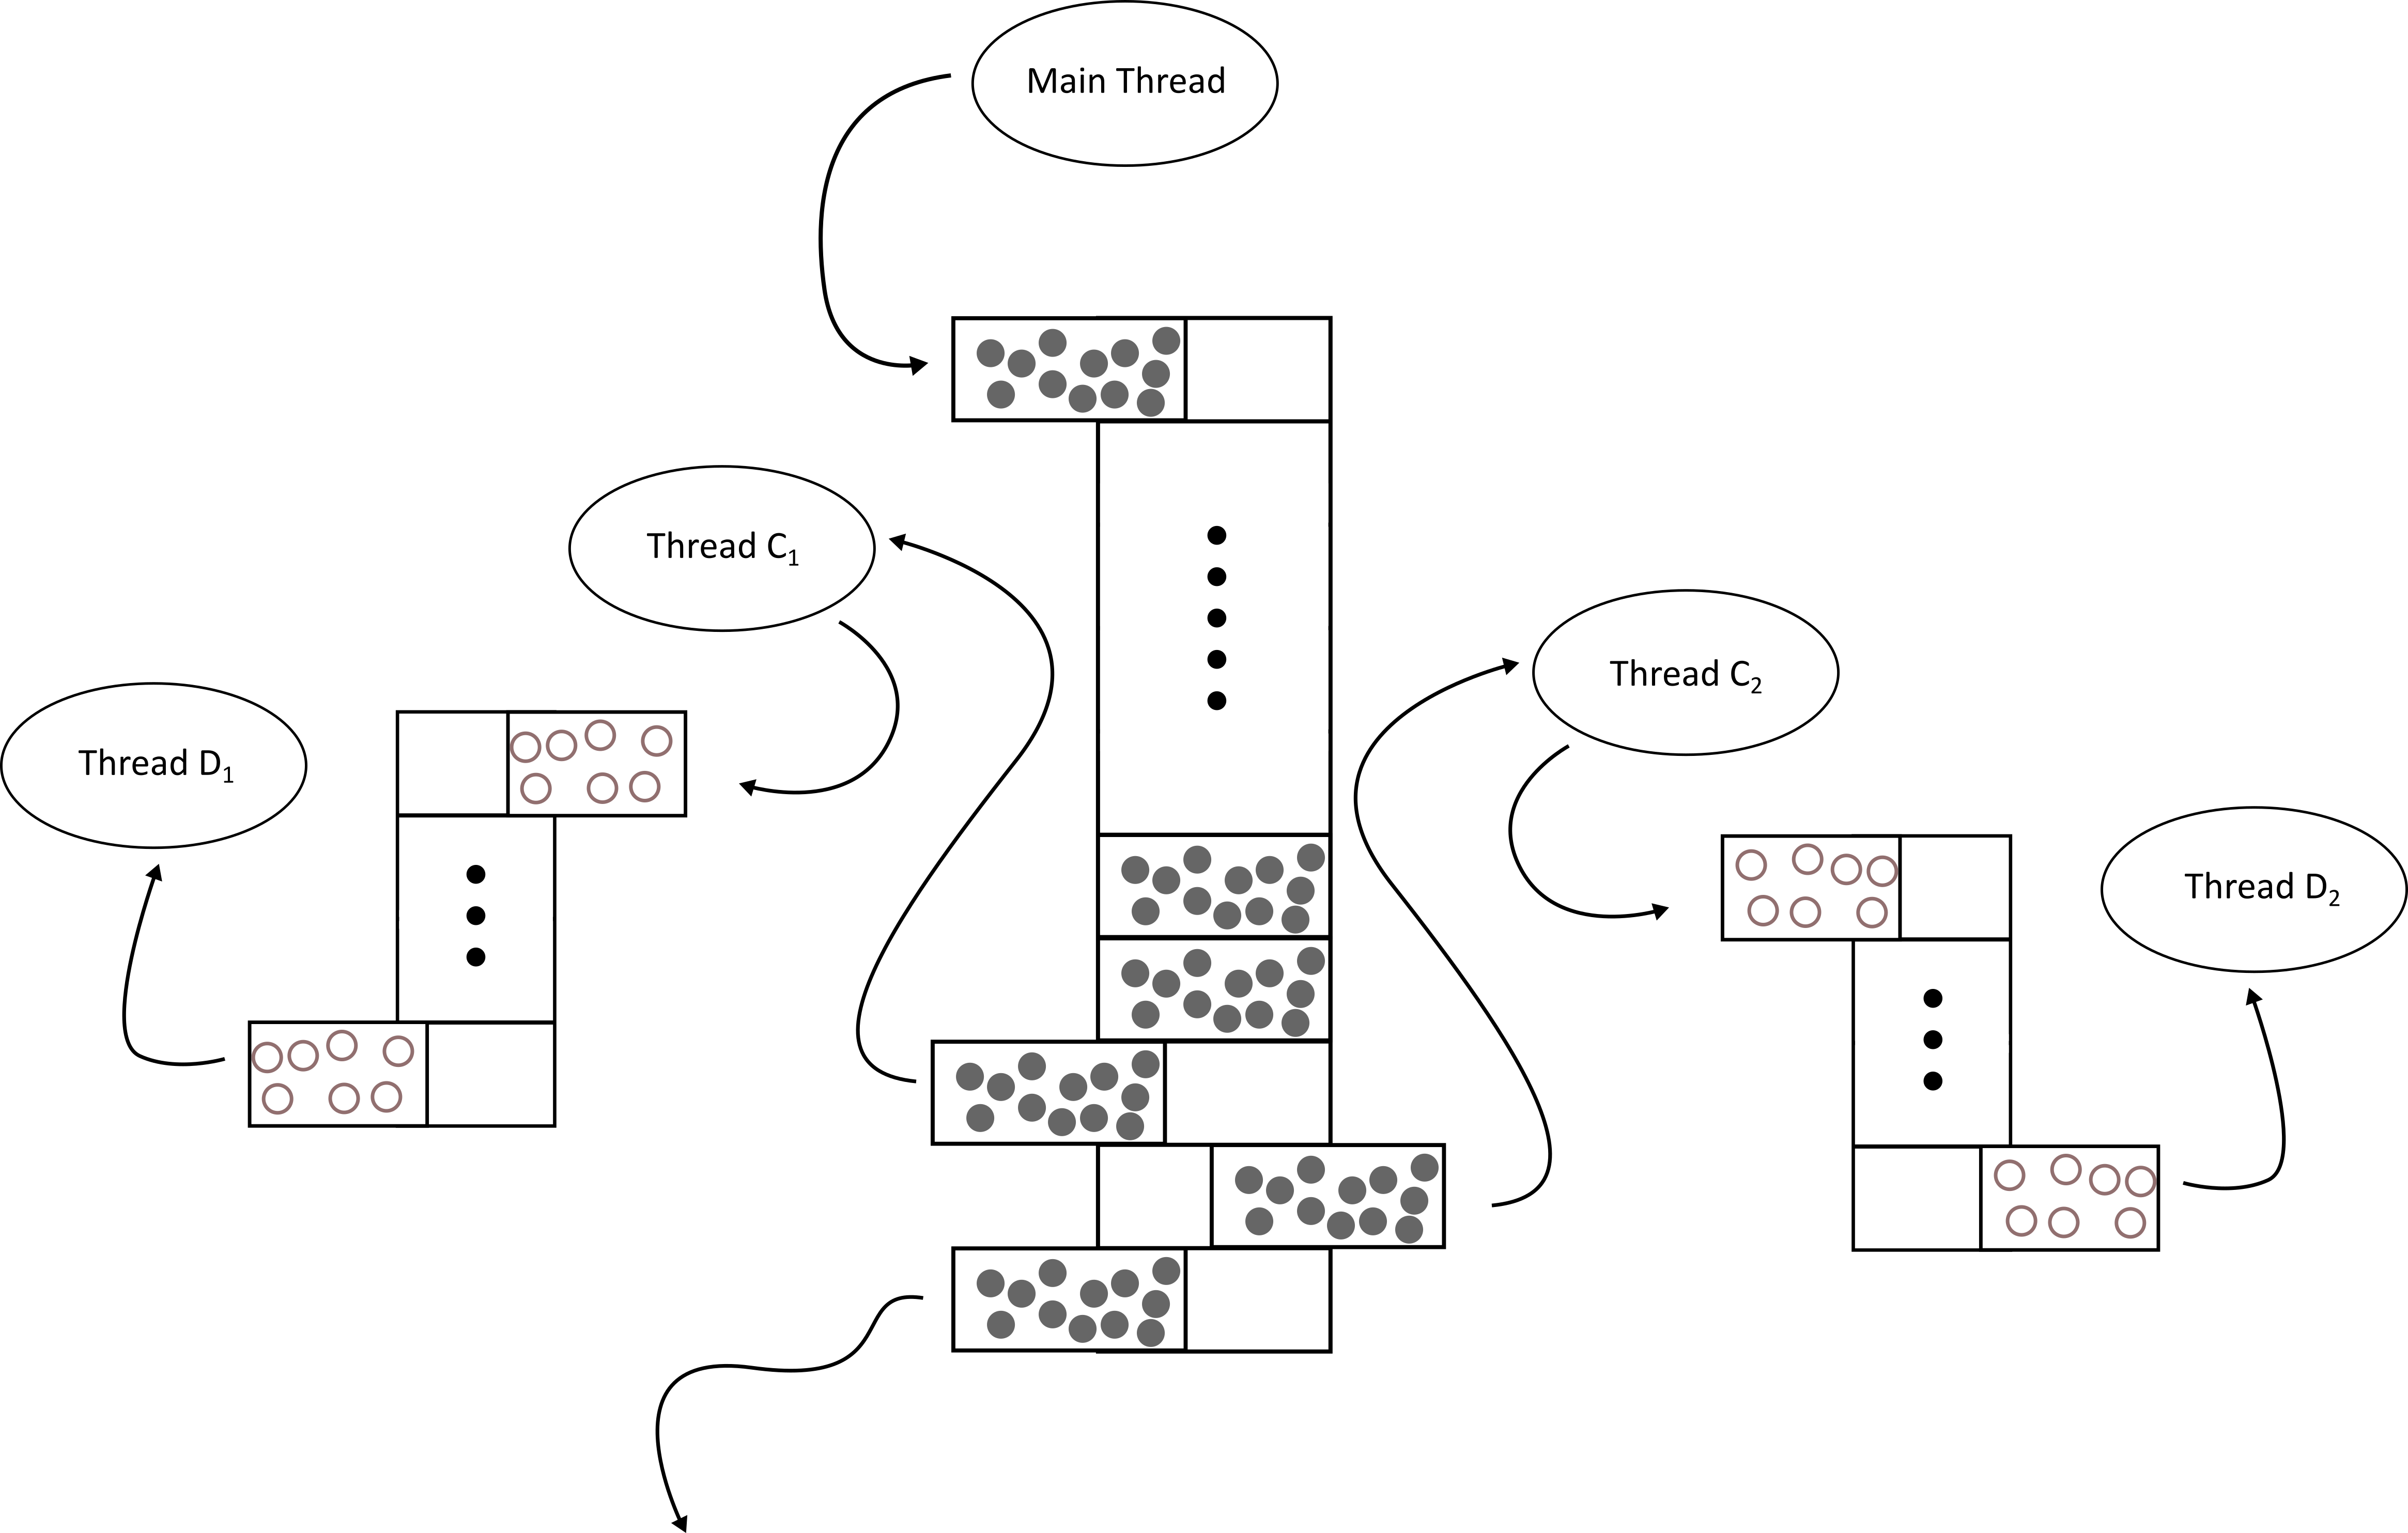
\includegraphics[width=\linewidth]{images/multithread.png}
    \footnotesize{Source: Made by the author.}
    \label{fig:multithread}
\end{figure}

\figref{fig:multithread} illustrates how the FP will be rearchitected in order to take advantage of parallel execution.
We can see that the main thread will collect the EGC for each cell grid and enqueue it in a shared queue that will be
acessed by $N$ consumers. Whenever a consumer ($c_t$ thread) dequeues an EGC, it will then try to find a pair of disks
for each pair of points in the EGC, cluster the remaining points in those disks and then enqueue those disks in another
shared queue. Such shared queue will only be shared with the disk thread $d_t$ belonging to the $c_t$ thread that
created it. Then, each $d_t$ will be responsible to check for subsets and supersets in its own set of disks, saving a
lot of processing time when those disks will be merged (and also checked for subsets and supersets) with the global disk
set in the \textsc{Process} procedure.
